The followed informations introduce the results of two different tests 
using the KITTI dataset\cite{Geiger}.


In the first test in Fig. \ref{fig:imgpapercerta}, 
the algorithm makes the tracking of an object through nine images in sequence with 
a displacement approximately perpendicular to the observer.
\begin{figure}[!hbt]
\centering
  \subfloat[]{\label{fig:imgpapercertaa} \includegraphics[width=.48\columnwidth]{images/images/0000000000.png}}
  \subfloat[]{\label{fig:imgpapercertab} \includegraphics[width=.48\columnwidth]{images/images/img_paper_certa.eps}}
  \caption{The image in (a) represents the target in its initial position 
   and the image (b) shows the vehicle in its final position.}
  \label{fig:imgpapercerta}
\end{figure}
The initial position of target is in the image (a) and the final position in (b), 
where a vector (in blue) illustrates the resulting trace.
We can observe that there is a small bend in the image 
and it generates a slight change of object perspective. 
This cause the update of the $ROI$, which involves seeing a slight change in area.
The difference among the initial and final values of the departure factor may 
be considered small, as shown in Fig. \ref{fig:res_graph1}.
\begin{figure}[!hbt]
\centering
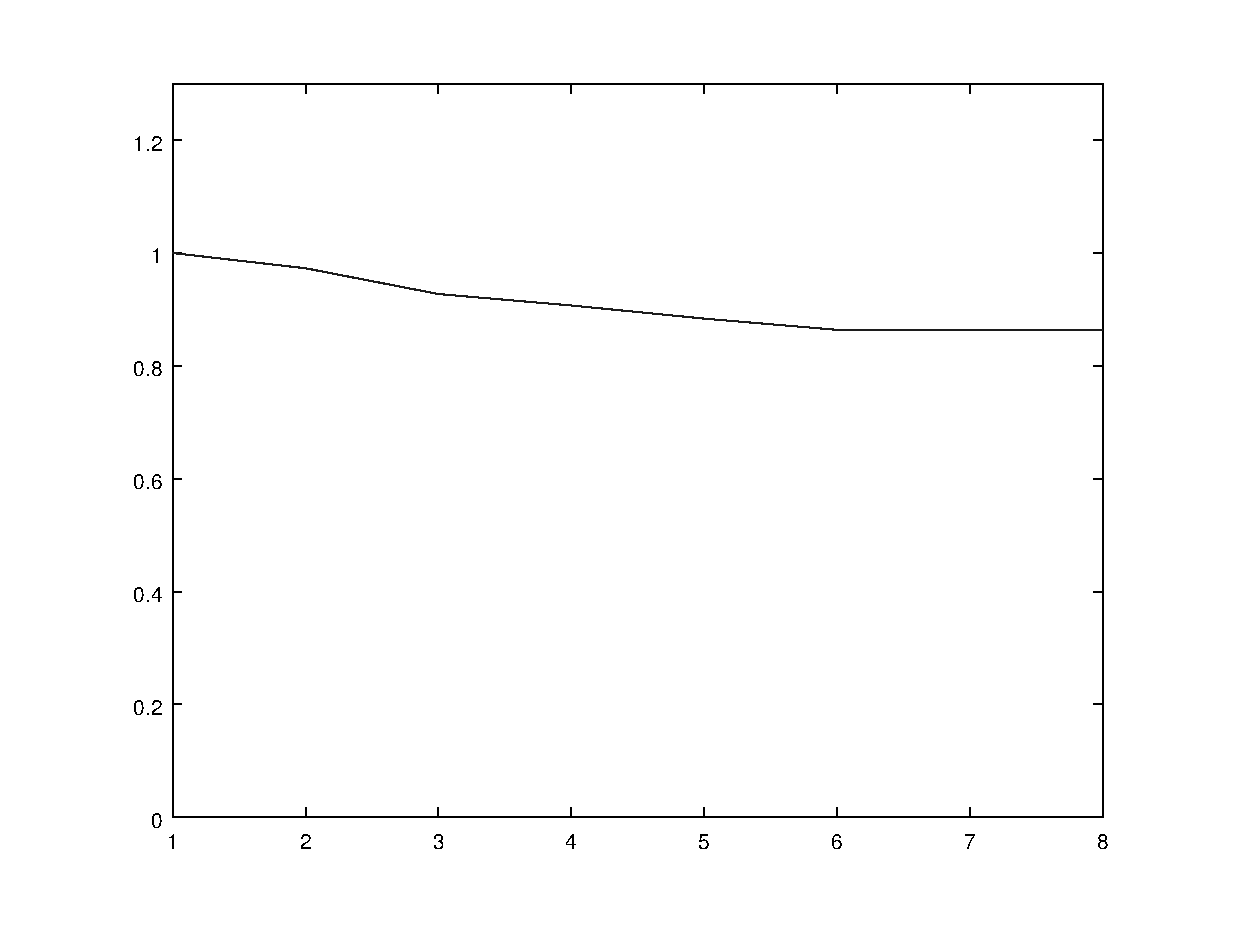
\includegraphics[width=0.8\columnwidth]{images/graph1.eps}
\caption{Departure factor for each frame in the test 1.}
\label{fig:res_graph1}
\end{figure}
Fig. \ref{fig:res_graph1v} shows the velocity of departure factor
to a value $d_0=1$ and a $\Delta t=1$. It demonstrates that the variation
of the departure factor is very small when compared with 1. 
It has a mean departure factor (velocity) of $-0.017020$. This implies in a mean approach of $1.7\%$ of $d_0$
in each one of the nine frames.
\begin{figure}[!hbt]
\centering
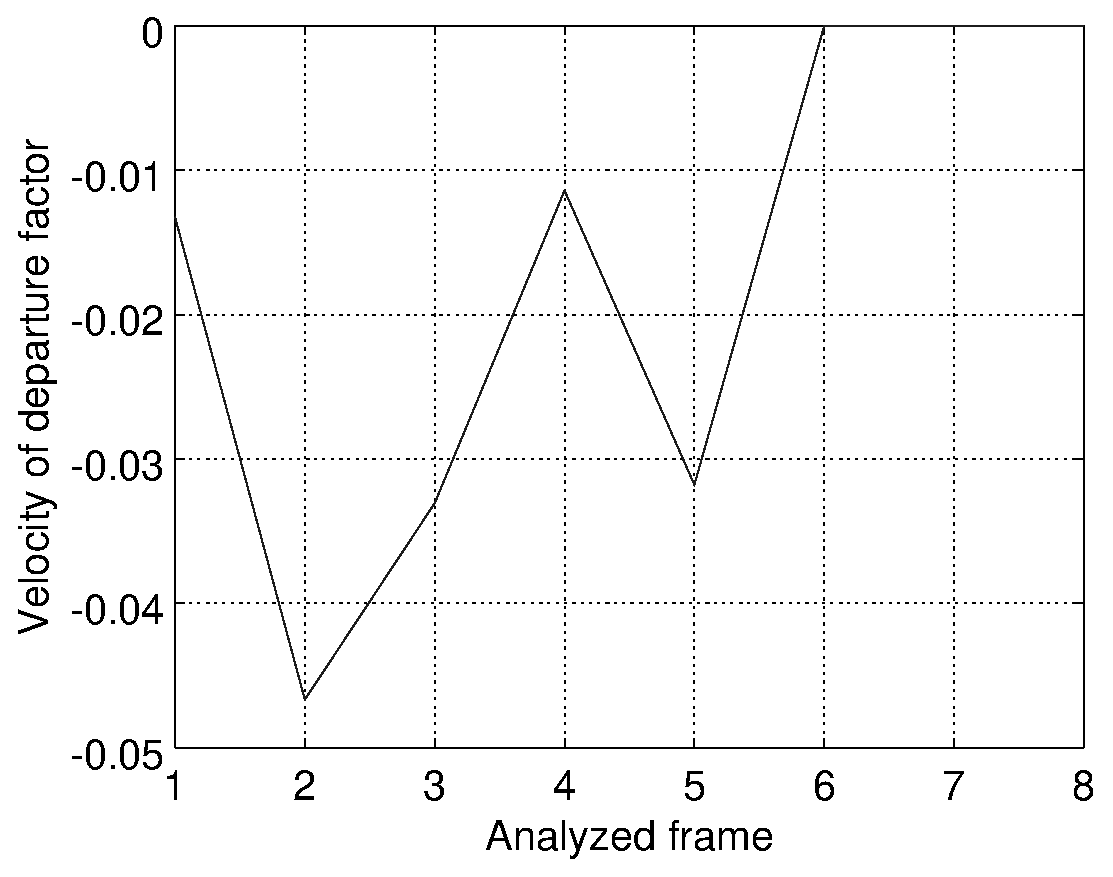
\includegraphics[width=0.8\columnwidth]{images/graph1v.eps}
\caption{Velocity of departure factor for each frame in the test 1.}
\label{fig:res_graph1v}
\end{figure}
